\section{Kontrolfunktioner}
\underline{\textbf{Controller klassen}}
\newline
Der blev valgt at samle programmets vigtigste funktioner i klassen \texttt{Controller}. Dette blev gjort for at user interface kun skulle i kontakt med én klasse, og fordi det ville blive nemmere i en senere iteration at implementere et Grafisk User Interface (GUI).
\newline
En af \texttt{Controller} klassens metoder er \texttt{sendBesked(besked, uName)}. Samarbejdsdiagrammet for \texttt{sendBesked()} er vist i figur \ref{fig:sendb}.
\begin{figure}[ht]
	\centering
	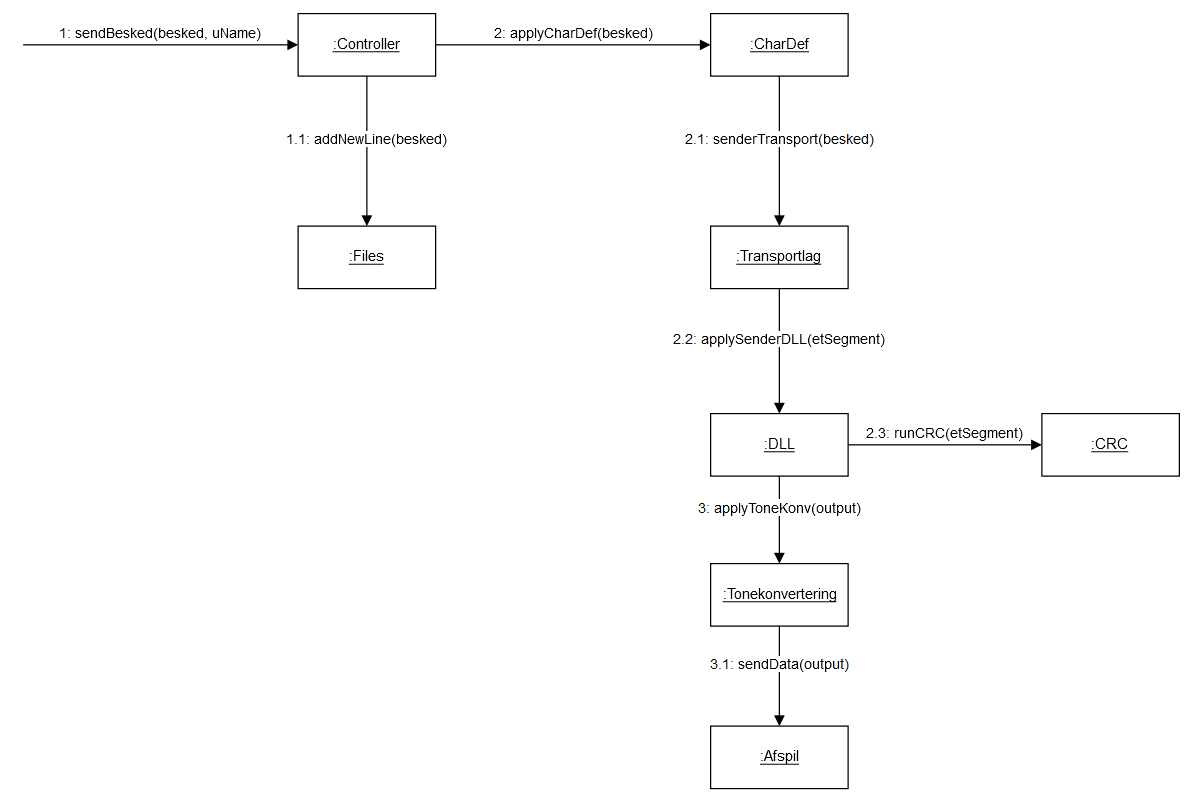
\includegraphics[width=15cm,height=25cm,keepaspectratio]{pictures/SDsend.png}
	\caption{\texttt{sendBesked()}}
	\label{fig:sendb}
\end{figure}
\hfill \break
Denne metode tager beskeden der skal sendes, samt navnet på den der har sendt den og samler det i en besked. Denne besked bliver sendt videre til \texttt{Chardefinition} klassen, som laver teksten om til en binær streng. Den bliver efterfølgende sendt til transportlaget, der kan dele beskeden op i mindre segmenter og sørge for at sendingerne foregår som de skal. Pakkerne vil kommere videre til Data Link Laget, hvor der vil blive tilføjet CRC og stuffing til bitstrengen. I \texttt{Tonekonvertering} bliver den binære streng omdannet til tal mellem 0 og 15, som er det antal toner der er til rådighed ved DTMF. Til sidst bliver tonerne afspillet med klassen \texttt{Afspil}. Når en besked er sendt, bliver den gemt i en fil med klassen \texttt{Files}.
\newline
Klassen har desuden en metode, der hedder \texttt{modtagBesked(uName)}. Samarbejdsdiagrammet for \texttt{modtagBesked()} er vist i figur \ref{fig:modtagb}.
\begin{figure}[ht]
	\centering
	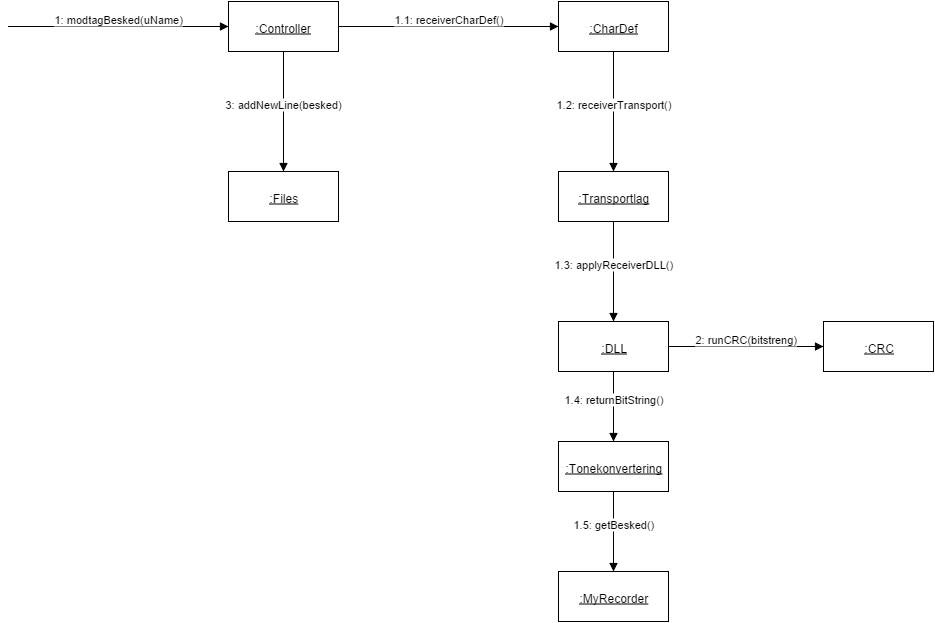
\includegraphics[width=15cm,height=25cm,keepaspectratio]{pictures/SDmodtagBesked.png}
	\caption{\texttt{modtagBesked()}}
	\label{fig:modtagb}
\end{figure}
\hfill \break
Denne går igennem de samme klasser som \texttt{sendBesked}, dog i stedet for at sende en besked afsted, sendes der en request om at modtage en besked. I klassen \texttt{MyRecorder} modtages beskeden, som returneres som toner af tal mellem 0 og 15 til \texttt{Tonekonvertering}'en, der omdanner tonerne til en bitstreng, som returneres til Data link laget. Ved \texttt{DLL} tjekkes for CRC og stuffing fjernes inden det returneres til transportlaget, hvor beskeden sættes sammen igen, hvis beskeden var delt op i segmenter. Den kommer retur til \texttt{CharDef} og bliver lavet fra binær streng til karakterer, som derefter returneres til \texttt{Controller}, der viser beskeden på skærmen og samtidig bruger \texttt{Files} til at gemme beskeden i en historik. Til dette bruges \texttt{uName} i metoden for at gemme i den rigtige historik.
\newline
\texttt{testLogin(uName, pWord)} er metoden der kan teste om et brugernavn og password er korrekt. Dette gør den ved at bruge \texttt{Login} klassen.
\newline
\texttt{createUser(uName, pWord)} bruger igen \texttt{Login} klassen, denne gang til at oprette en bruger. Samarbejddiagrammet er vist i figur \ref{fig:createu}.
\begin{figure}[ht]
	\centering
	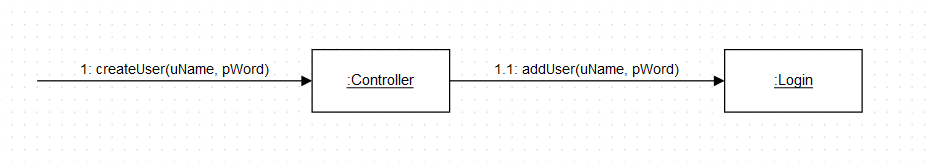
\includegraphics[width=15cm,height=25cm,keepaspectratio]{pictures/SDcreateUser.png}
	\caption{\texttt{createUser()}}
	\label{fig:createu}
\end{figure}
\hfill \break

Der er også metoder der kan vise historikken. De bruger alle \texttt{Files} klassen og kan enten vise hele historikken, sidste besked eller en der kan definere hvor mange linjer der skal hentes og vises.

\hfill \break
\underline{\textbf{Login klassen}}
\newline
Klassen \texttt{Login} bruges til at oprette og teste brugernavn og password. Metoden \texttt{addUser(uName, Pword)} opretter nye brugere og gemmer brugernavn og password i et txt dokument.
\newline
Klassen har også metoden \texttt{testLogin(uName, pWord)}, som bruger metoden \texttt{validateLogin(uName, pWord)}. Den modtager et brugernavn og login, som bliver lavet om til en string. Denne string bliver efterfølgende sammenlignet med alle de brugernavne og passwords der er gemt i txt filen. Hvis der ikke findes et match bliver der returneret true og brugeren logges på.

\hfill \break
\underline{\textbf{Files klassen}}
\newline
\texttt{Files} klassen bruges til at gemme historik, når der bliver skrevet til hinanden med chat programmet. Files virker ved at når der oprettes et objekt at klassen, med en parameter, som er brugernavnet, bliver der oprettet et txt dokument med brugerens navn, som historikken kan gemmes i.
\newline
Funktionen \texttt{addNewLine(besked)} tilføjer en besked til tekstdokumentet. \texttt{updateVector()} bruges til at lave en vektor af linjerne fra historikken, som efterfølgende evt. kan printes ud på en skærm så brugeren kan se indholdet. Der er en metode \texttt{clearText()}, der kan slette alt fra historikken. Der er også metoden \texttt{printVector()}, der kan printe hver linje ud, som er i vektoren skabt med \texttt{updateVector()}. \texttt{printLatest()} printer den sidste besked ud og \texttt{printLines(startN, endM)} kan printe de valgte linjer ud fra linje n til m. Til sidst er der en metoden flipVector(), den bruges til vende vectoren, så fx den sidste modtagne besked kommer til at ligge øverst i vektoren, altså på plads 0.

\hfill \break
\underline{\textbf{CharDefinition klassen}}
\newline
\texttt{CharDefinition} klassens opgave er at omdanne forskellige karakterer om til binærer tal og tilbage igen. Hvis der oprettes et objekt af klassen, bliver der skabt en string af alle de tal, karakterer og andre tegn der tænkes at skulle kunne sendes. Den string kan bruges i metoderne. Der er en metode som hedder \texttt{applyCharDef(input)}, der bruger en anden metode \texttt{charToBinary}, som kan omdanne karakterer i en besked til binær, inden den sendes videre til Tranportlaget.
\newline
\texttt{charToBinary(input)} metoden tager inputtet som er en string af karakterer og laver det om til en binær string. Det gør den ved at kigge på de karakterer, der skal sendes og sammenligne dem med de definerede karakterer og tegn. Hvis der findes et match, bruges nummeret på placeringen af karakteren i den definerede string, som den binære værdi. Den binære værdi bliver 8 bits lang. Fx karakteren b, som har placeringen 12, får binær værdien 00001100.
\newline
\texttt{receiverCharDef()} er metoden der bruges når der returneres beskeder fra transportlaget og laver beskeden om fra binær til karakterer. Hvis beskeden der modtages er en fejlbesked sende den videre og vises på skærmen. Ellers bruges metoden \texttt{binaryToChar(messageReceived)} der omdanner de otte bits om til et decimaltal, som igen kan bruges til at finde placeringen af karakteren, der er modtaget og derefter sætte det på en string. Det gøres indtil hele beskeden er omdannet.

\hfill \break
\underline{\textbf{UI source}}
\newline
Til chat programmet er der valgt at lave et simpelt user interface. Det blev lavet ved at bruge konsolvinduet i Visual Studio. Et flowdiagram af systemet er vist på figur \ref{fig:uif}.
\begin{figure}[ht]
	\centering
	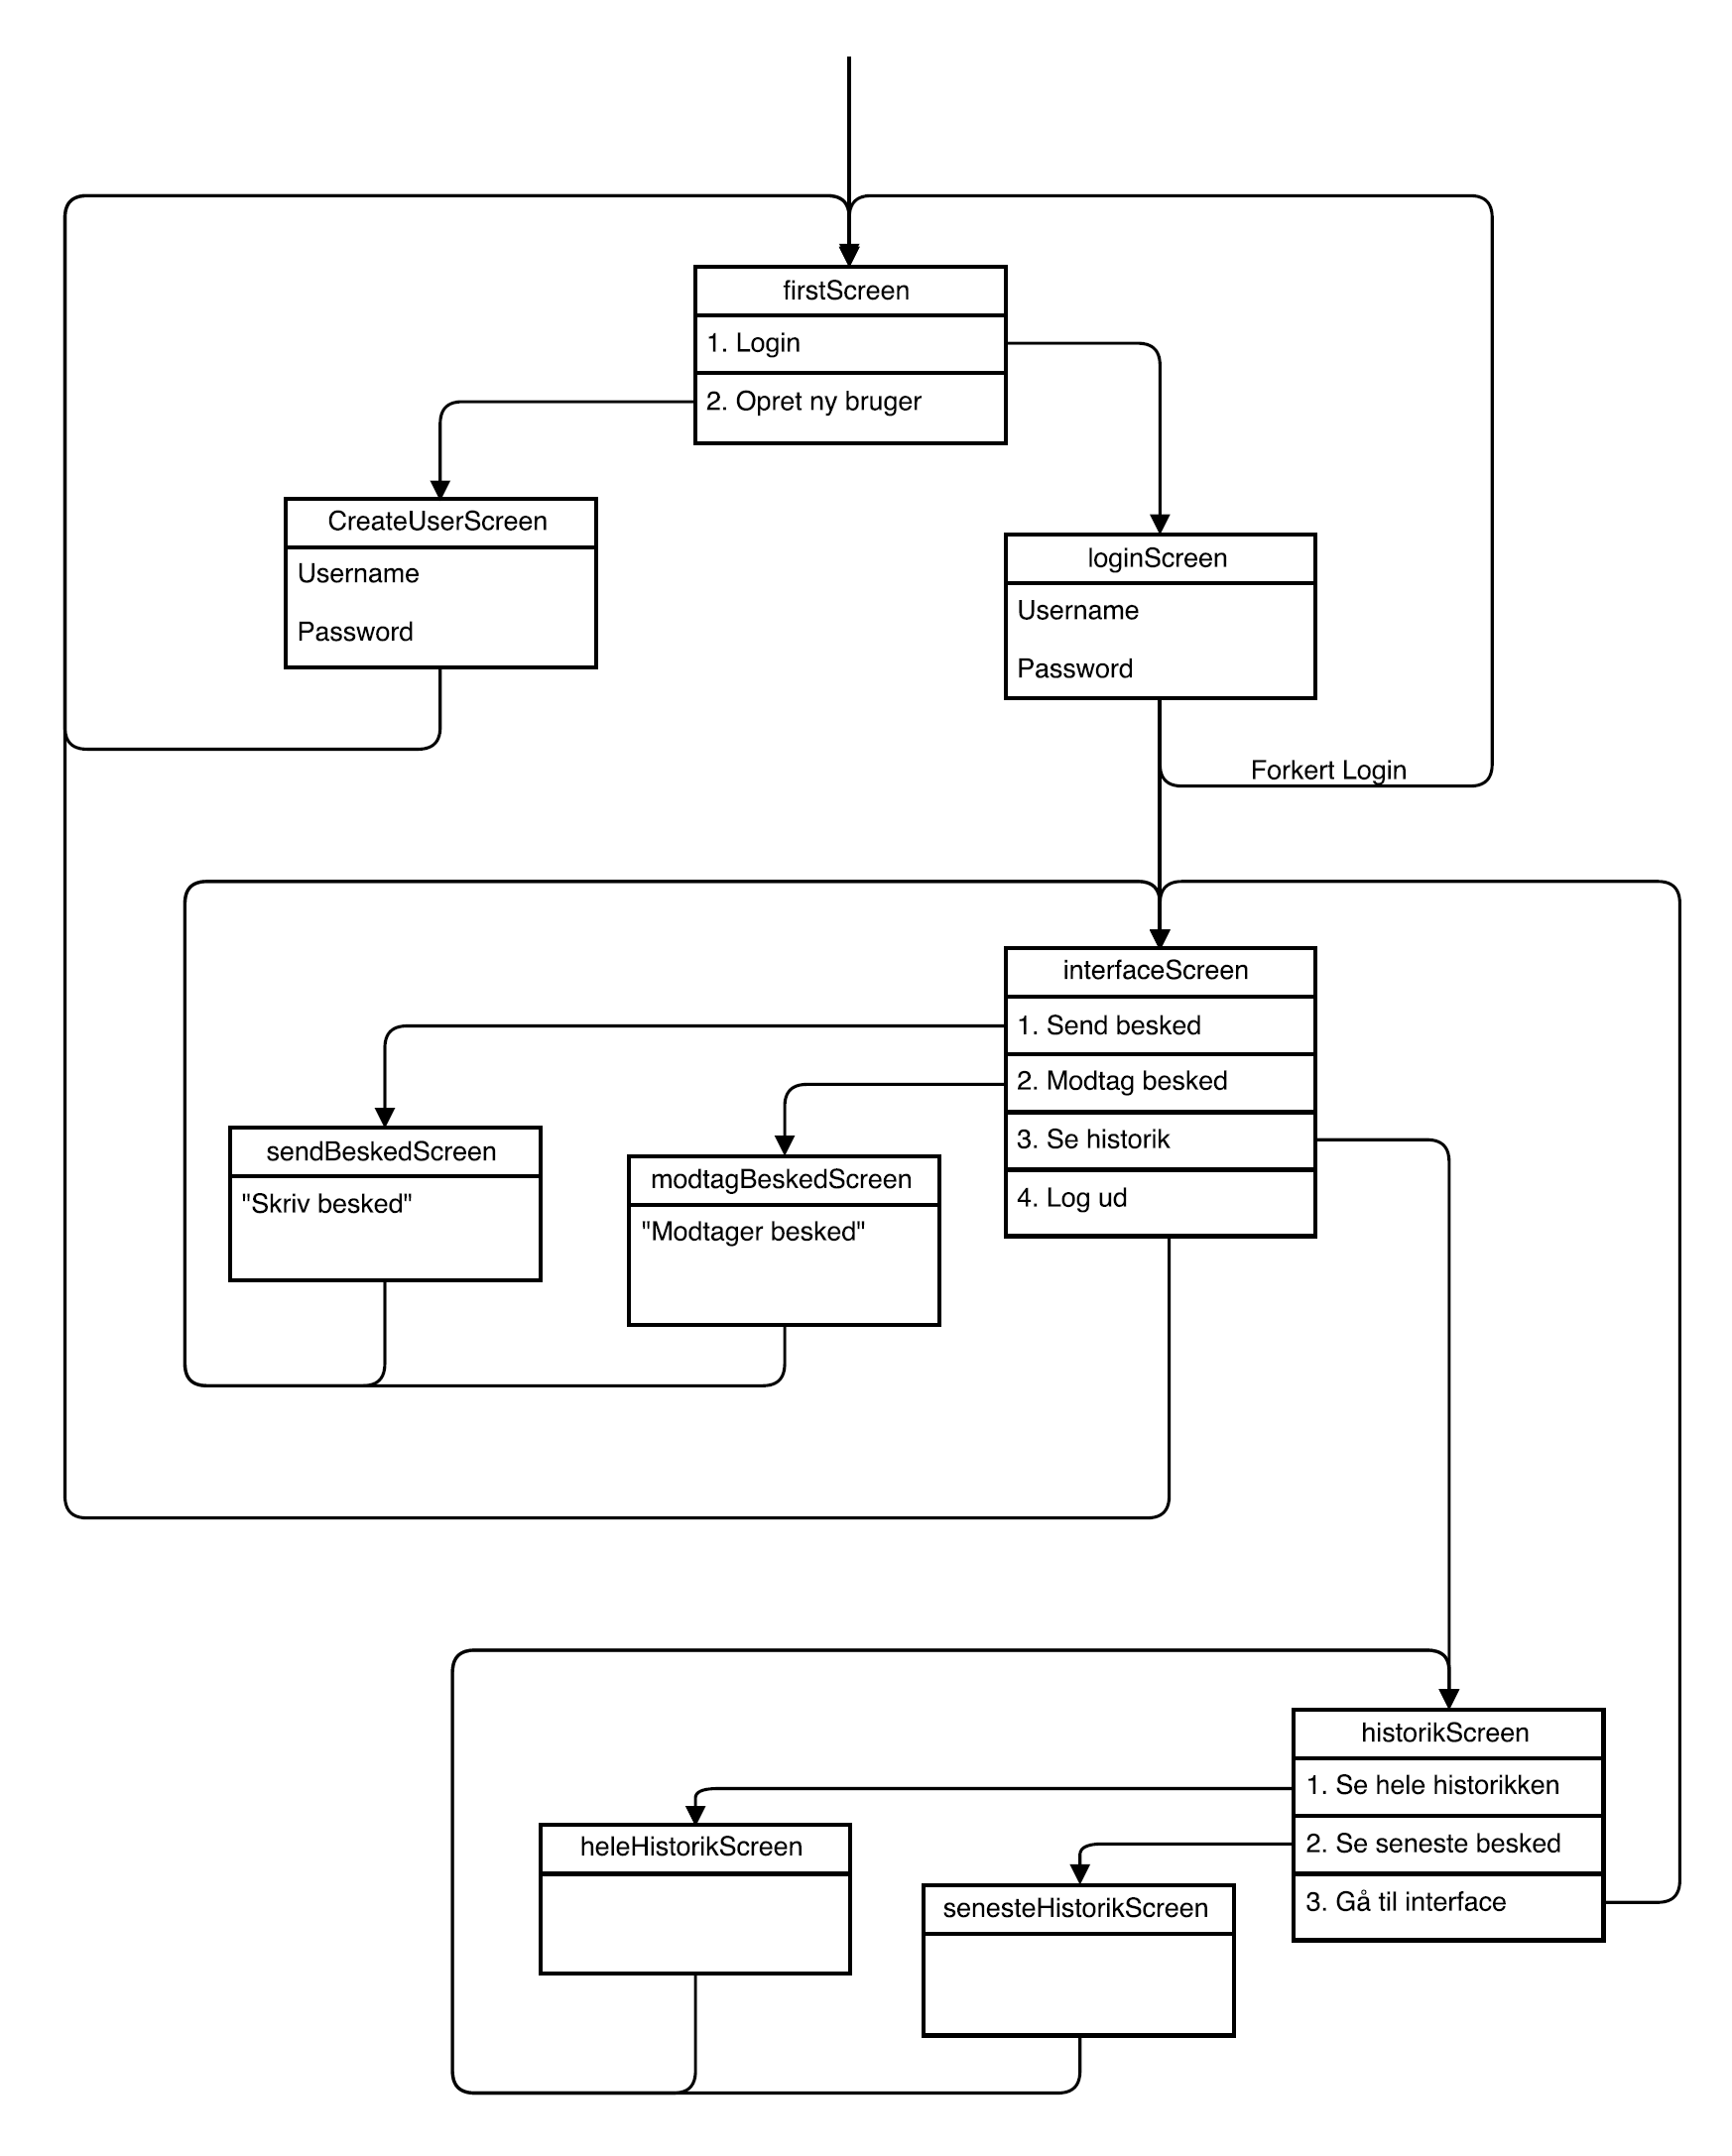
\includegraphics[width=15cm,height=25cm,keepaspectratio]{pictures/UIflow.png}
	\caption{\texttt{UI flowdiagram}}
	\label{fig:uif}
\end{figure}
Programmet er bygget op ved at der gives nogle valgmuligheder. På første skærm kan der vælges mellem login eller opret bruger. Der vælges ved at indtaste et tal, her 1 eller 2. Tallet sammenlignes med de muligheder der er og programmet går til næste skærm. Når der oprettes ny bruger, indtastes brugernavn og password som efterfølgende bruges i \texttt{Controller} klassen i metoden \texttt{createUser(uName, pWord)}. Der vil efterfølgende gås videre til loginskærmen, hvor brugernavn og password indtastes igen og bruges i metoden \texttt{testLogin(uName, pWord)}. Hvis det indtastede er forkert kan der prøves igen ellers kommer interface skærmen. Her er mulighederne: Send besked, modtag besked, se historik og log ud. Ved send besked skærmen kan der skrives en besked, som efterfølgende sendes med metoden \texttt{sendBesked(besked, uName)}. Ved modtagBesked skærmen afventes der en besked. Den modtages med metoden \texttt{modtagBesked()} og bliver efterfølgende vist på skærmen. Hvis der vælges historik, kommer en skærm med 3 muligheder igen. Her kan der vælges at se hele historikken eller seneste besked som vises med metoderne \texttt{getHeleHistory()} og \texttt{getSenesteHistory()}. Den sidste valgmulighed er retur til interface skærmen.